\documentclass[a4paper]{article}

\usepackage{ReportTemplate}

\usepackage{setspace}
\usepackage{amsmath}
\usepackage[hidelinks]{hyperref}

\title{Project 1:基于线性分类器和语音短时特征的简单语音端点检测}
\name{薛春宇}
\studentid{518021910698}

\begin{document}

\maketitle

\begin{abstract}
    \textit{语音端点检测 (Voice Activity Detection) 的目的是对连续语音信号中语音和非语音的区域进行区分,其准确性直接影响到整个语音识别系统的性能。本项目中基于线性分类器的VAD算法将语音检测视作二分类问题,通过语音的短时时域/频域特征构造特征向量,使用逻辑回归模型构建分类器,并基于dev开发集进行训练和AUC、EER指标评估,采用简单状态机架构以达到端点检测的目的。综合其在test测试集上的表现得出,该模型为语音端点检测提供了一个简单高效的方案。} 
\end{abstract}

\textit{
\textbf{Keyword:} 语音端点检测,语音短时特征,逻辑回归模型,指标评估,简单状态机
}


\section{Introduction}

语音端点检测 (VAD) 通过对连续语音信号中的语音/非语音区域进行探测和标注,为后续语音识别的准确性提供了坚实的基础。准确可靠的VAD可以减少语音识别系统的计算量和能耗需求,进而改善上层系统的性能[\ref{ref1}]。大多数VAD系统通过监控一个指标,并将其与设定好的阈值作比较,以此观察该信号是否为语音信号。

本文首先在第2节中介绍一些用于构建特征向量的语音短时时域和频域特征,其中,时域特征包括短时能量 (Short Time Energy) 和短时过零率 (Zero-crossing Rate),频域特征包括短时频谱 (Short Time Spectrum) 和梅尔频率倒谱系数 (Mel-Frequency Cepstral Coefficients),上述特征均具有“短时平稳”的特性。基于上述特征,本文将在第3节中使用机器学习的方法构建了一个逻辑回归线性分类器,并在dev开发集上进行模型训练和包含AUC和EER等指标在内的指标评估。在上述线性分类模型之上,本文会在第4节通过简单有限状态机的方式,实现针对不同语音信号进行端点检测的目标。第5节中,在test测试集上的实验结果表明,该VAD模型在不同声音、不同背景噪声之下,均具有较好的端点检测能力。

\section{语音短时特征}

语音信号为短时平稳信号,加窗分帧后具有“短时平稳”的性质,这为我们构造特征向量,训练分类器提供了理论支持。一般采用10 - 30ms 的帧长(本项目选择30ms 作为帧长)。对于语音短时特征的分析又可以分为时域和频域两个方向。

短时时域特征主要体现语音信号一些能量、清浊上的特征,典型代表是短时能量STE和短时过零率ZCR,前者是语音信号一帧内采样点的平方和,后者是一帧内信号正负反复的次数。

短时频域特征则主要体现语音信号频率、能量分布方面的特征,典型代表是短时频谱STS、基频FF和梅尔频率倒谱系数MFCC。其中,短时频谱是逐帧进行短时傅里叶变换STFT,再取最高峰所对应的频率作为特征指标的。基频的估算则是通过YIN算法实现的,其核心思想仍是自相关法,但由于其计算量如图\ref{fig:1}所示相较于其他频域特征显著大,因此本项目中并未采取基频作为特征指标。

\begin{figure}[htb]
  \centering
  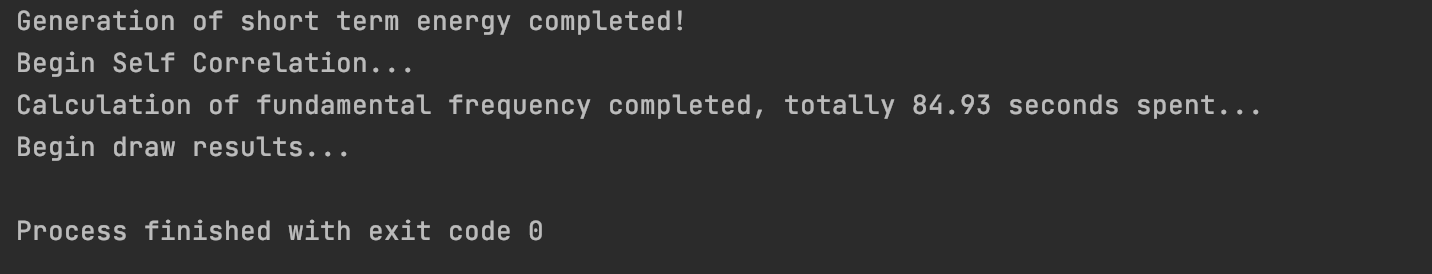
\includegraphics[scale=0.3]{figs/fundamental_frequency_1.png}
  \caption{基频计算量(单个wav 84.93s)}
  \label{fig:1}
\end{figure}

频域特征之一的梅尔频率倒谱系数MFCC包含两个步骤,分别是将语音信号转化为梅尔频率,和进行倒谱分析,其物理意义可以理解为语音信号能量在不同频率范围的分布。由于本次端点检测任务较为简单,只需选取前13个梅尔系数作为特征指标即可。

\section{基于Logistic Regression逻辑回归的线性分类器}

本节中,我们将介绍包含数据预处理、特征提取、分类器算法、指标评估在内的完整开发流程。

\subsection{数据预处理及特征提取}

本项目使用VAD数据集对分类器的进行训练和测试,其中分为dev开发集、test测试集和train训练集三个子数据集,本模块主要使用dev开发集对分类器进行训练和评估。

开发集分为wav格式的数据文件和对应的标签两个部分,在读入前会针对文件名分别进行字典排序,从而保证数据和标签对应关系的正确性。对于wav文件,我们首先将声音信号进行归一化、加窗分帧(注意,本项目在语音信号加窗分帧的步骤中选择的帧长统一为30ms,帧移为15ms)等基本操作,随后逐帧进行STE、ZCR、MFCC等短时特征的计算,并将这些特征值合并为特征向量,与该wav文件内的帧进行一一对应。对于标签文件,我们首先逐行读取txt文件,进行起始时间点的格式划分,并将语音端点根据已有的帧长、帧移从以时间为单位对应到以帧为单位,并将位于起止端点内的帧全部打上1的标签,代表这些帧内均存在语音事件。

由于单次对整个数据集进行特征提取仍会花费较长时间,我们选择将上述方法生成的特征向量和相应的标签分别保存为"./input/features/dev\_features.npy" 和“./input/labels/dev\_labels.npy”,以便之后在模型训练、评估和预测中直接调用。

\subsection{逻辑回归分类器算法}

本模块中,我们首先从保存路径中读取经过预处理得到的特征向量和标签,并将所有wav文件的特征向量组合成一个纬度为 $n \times 1$ 的特征向量一维列表,其中 $n$ 为dev开发集中所有wav文件帧数目的和。对于标签集也进行相同的操作,注意到此时帧和标签仍保持一一对应的关系。随后,我们选取 $t$ 个权重 $[w_1, w_2, ..., w_t]$作为权重向量 $\hat w$,作为逻辑回归分类器的内部参数,注意到 $t$ 对应特征向量的维数,这里的值为16 ($STE + ZCR + STS + 13 \times MFCC$)。

Logistic分布函数的数学表达式如式\ref{eq:logistic}:
\begin{equation}
  F(x) = P(X \leq x) = \frac{1}{1 + e^{-(x-\mu)/\gamma}}
  \label{eq:logistic}
\end{equation}

其中,$\mu$表示位置参数,$\gamma > 0$为形状参数。在考虑二分类问题时,我们可以利用上述权重向量$\hat w$,基于Logistic分布函数的非线性来构造逻辑回归模型,如式\ref{eq:logistic2}:
\begin{equation}
 P(Y=1/x) = \frac{1}{1 + e^{-(\hat w^Tx+b)}}
  \label{eq:logistic2}
\end{equation}

上述模型表示输出$Y=1$的对数几率由输入$x$的线性函数表示,$\hat w^Tx+b$的值越接近正无穷,$P(Y=1/x)$的概率越接近1。由上得出,逻辑回归的思路是先拟合决策边界,再建立这个边界与分类的概率联系,从而得到二分类情况下的概率。

随后,我们对逻辑回归模型进行额外优化设置:$L2$ 正则化、正则化系数的倒数 $C=0.001$,并选择liblinear作为损失函数的优化方法,其内部使用了坐标轴下降法来迭代优化损失函数。这样的选择是基于和sag、saga、lbfgs等优化方法的效果对比后得出的,事实证明liblinear速度显著更快,更适用于数据集较小下的逻辑回归。

设置好逻辑回归模型及相关优化参数之后,我们开始模型训练:将处理后的 $n \times 1$维特征向量列表作为模型的输入,得到预测结果后与相应的标签的进行比对计算损失函数,并利用liblinear优化的坐标轴下降法迭代优化损失函数,当模型收敛后停止训练。注意,上述步骤在代码实现中均集成在sklearn.linear\_model.LogisticRegression下的.fit()函数中。完成训练后,我们在逻辑回归模型后面添加一定的后处理步骤,包括中值滤波和基于阈值的二值化,进而使得模型的预测结果成为指示哪一帧为语音帧的二值序列。

本模块的核心代码结构如下:

\begin{lstlisting}[language=python]
# 读取预处理后的特征向量和标签
features_vector_list = read([features_path])
labels_list = read([labels_path])
# 生成模型训练用的n*1维的batch
dev_X, dev_Y = generate_batch(features_vector_list, labels_list)
# 设置模型参数
model = sklearn.linear_model.LogisticRegression([parameters setting])
# 模型训练
model = model.fit(dev_X, dev_Y)
# 预测结果,test_X为一个wav文件生成的帧序列的特征向量列表
pred_Y = model.predict_proba(test_X)
# 模型后处理:中值滤波+阈值二值化
pred_Y = medfilt(pred_Y, kernel_size)
for i in range(len(pred_Y)):
    if pred_Y[i] == 0:
        # Silence State
        continue;
    # Speech or Noise State
    pred_Y[i] = 1 if pred_Y[i] > voice_threshold else 0
# 返回预测结果
return pred_Y
\end{lstlisting}

\subsection{指标评估}

本模块中我们将介绍在上述模型训练完成后,利用ROC曲线下的面积AUC和等错误率EER指标来进行模型正确性评估的方法。ROC曲线即接受者操作特征曲线,指在特定刺激条件下,以受试者在不同判断标准下所得的误报率FPR为横坐标,召回率TPR为纵坐标得到的曲线,值越大说明模型越好。EER等于ROC上FPR和TPR相同时的取值,值越小说明模型越好。

本模块的具体实现方法是,遍历dev预处理得到的特征向量集及相应的标签集,每次计算单个特征向量的AUC和EER并存储,最后返回整个特征向量集的平均AUC和EER作为统计指标。具体的计算过程被封装在get\_metrics()函数中,通过skearn.metrics方法下的roc\_curve和auc函数实现。本模块的核心代码结构如下:

\begin{lstlisting}[language=python]
# AUC和EER各自的和
total_auc = 0
total_eer = 0
# 遍历特征向量集和标签集
for i in range(len(features_vector_list)):
    # 计算当前AUC和EER
    cur_auc, cur_eer = get_metrics(features_vector_list[i], labels_list[i])
    # 统计
    total_auc += cur_auc
    total_eer += cur_eer
# 返回均值
return total_auc/len(features_vector_list), total_eer/len(features_vector_list)
\end{lstlisting}

经过指标评估,本模块运行结果如图\ref{fig:2}所示,最终得到的$AUC = 0.9407$,$EER = 0.1044$。

\begin{figure}[htb]
  \centering
  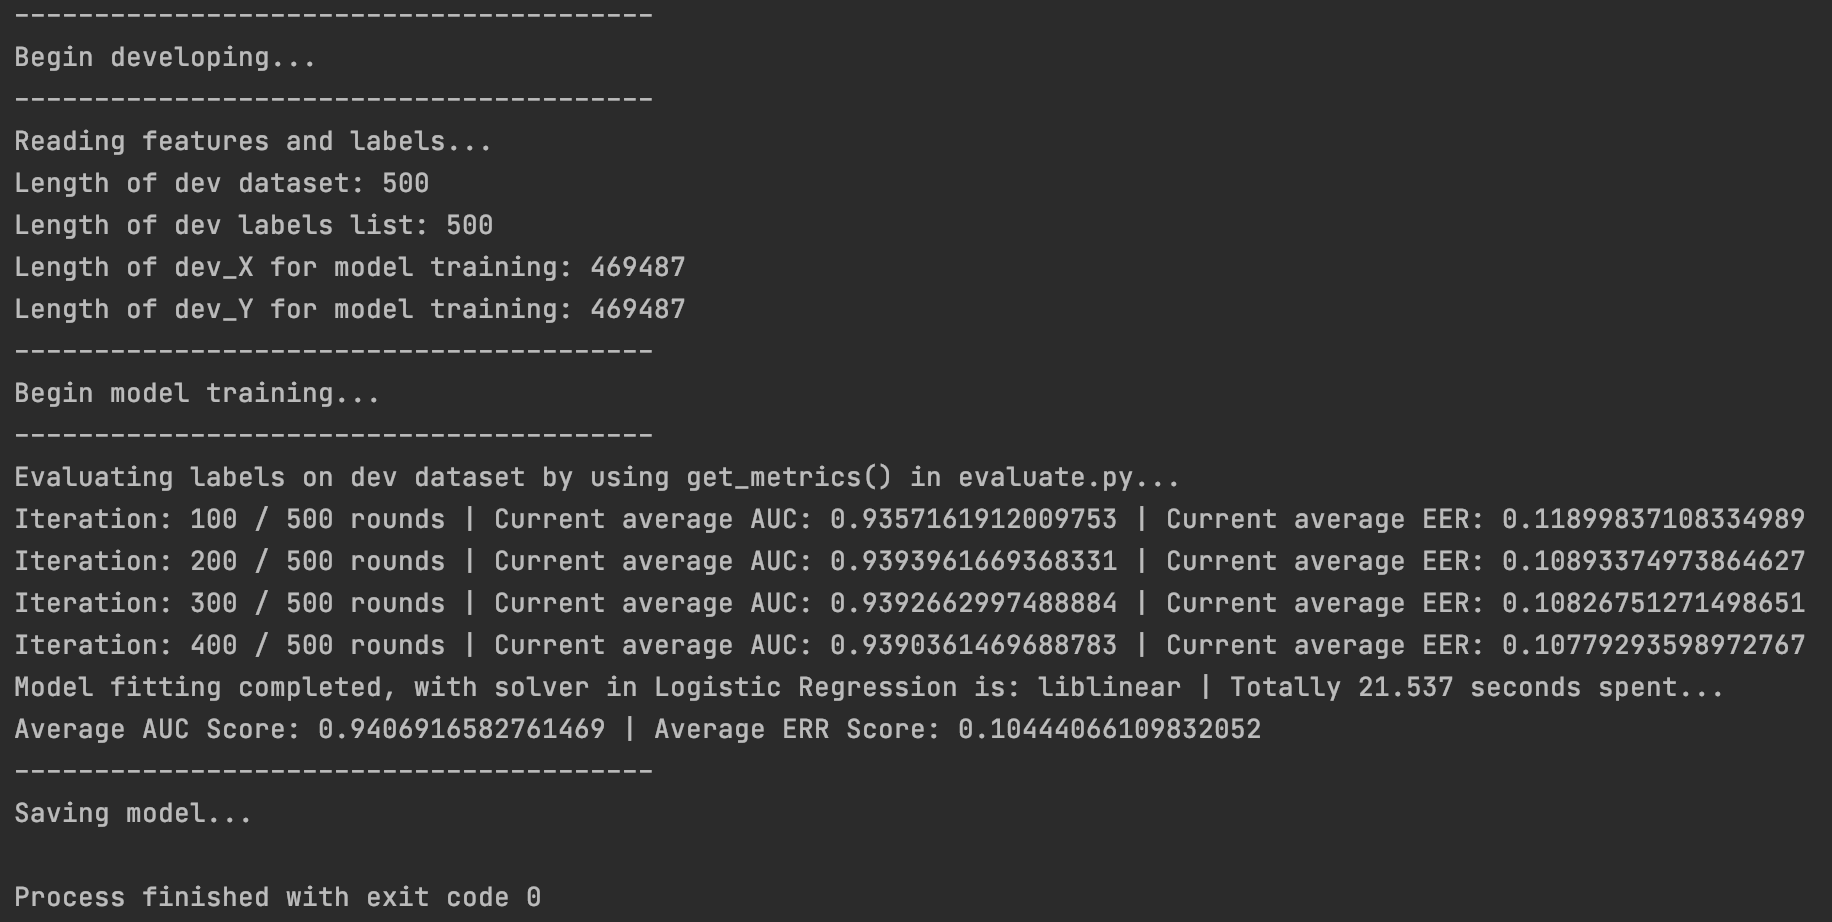
\includegraphics[scale=0.25]{figs/评估(平滑+二值化.png}
  \caption{dev开发集指标评估结果}
  \label{fig:2}
\end{figure} 

单独取dev开发集字典排序后的第一个wav文件,绘制ROC曲线如图\ref{fig:4}:

\begin{figure}[htb]
  \centering
  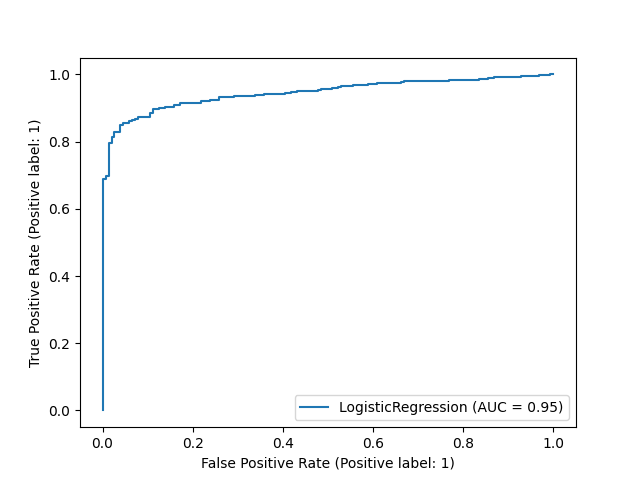
\includegraphics[scale=0.5]{figs/roc_curve_1.png}
  \caption{ROC接受者操作特征曲线}
  \label{fig:4}
\end{figure} 

为了进一步探索模型后处理(平滑和二值化)对AUC和EER指标的影响,我们针对预测结果是否进行中值平滑和是否进行阈值二值化处理进行了一系列的对比实验,结果如表\ref{tab:tab1}:

\begin{table}[th]
  \caption{指标评估影响因素对比实验}
  \label{tab:tab1}
  \centering
  \begin{tabular}{ l c c c r }
    \toprule
    \textbf{ } & \textbf{G1} & \textbf{G2} & \textbf{G3} & \textbf{G4} \\
    \midrule
    AUC & 0.9407 & 0.9886 & 0.9019 & 0.9649 \\
    EER & 0.1044 & 0.0381 & 0.1665 & 0.0793 \\
    \bottomrule
  \end{tabular}
\end{table}

其中,G1表示同时进行平滑和二值化,G2表示仅平滑,G3表示仅二值化,G4表示不经过处理。基于上述结果得出结论:对预测得到的概率数组进行中值平滑有利于提高预测准确率,而进行阈值二值化会造成AUC和EER指标的降低。然而,为了进行语音端点预测,我们必须将概率数组进行二值化,因此针对预测结果包括中值滤波在内的后处理十分重要。注意,上述指标评估和模型训练均基于dev开发集,在第5节中会在test测试集中进行额外的指标评估,以验证模型的正确性。

\section{基于LR线性分类器的简单有限状态机}

有限状态机是一种用来进行对象行为建模的工具,其作用主要是描述对象在其生命周期内所经历的状态序列,以及如何响应来自外界的各种事件。本节将介绍基于上述理论实现的Logistic Regression线性分类器,对语音端点检测中的事件进行抽象化,构建简单的有限状态机FSM,如图\ref{fig:3}所示。

\begin{figure}[htb]
  \centering
  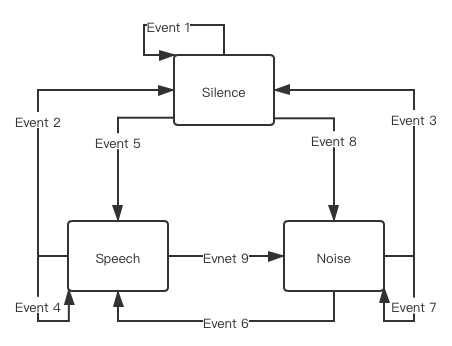
\includegraphics[scale=0.5]{figs/FSM.png}
  \caption{FSM的状态转移关系}
  \label{fig:3}
\end{figure} 

本模型的有限状态机共包含3个状态,分别为Slience、Speech和Noise。该有限状态机的输入为逻辑回归分类器的预测结果(逐帧输入),每一个输入代表分类器判断该帧是否为语音帧的可能性。对于当前第i帧,上一帧的位置决定先前位于哪一个state(若i=1则默认位于Silence state)。输入第i帧的预测结果pred\_Y[i],记为p。若p=0,触发Event 1/2/3;若voice\_threshold<p<=1,触发Event 4/5/6;否则触发Event 7/8/9。若位于Silence或Noise状态,则输出0,表示该帧非语音帧;否则输出结果1。

\section{实验和结果}

本节分为两个部分,分别是基于部分train训练集的模型评估,以及基于test测试集的语音端点预测。

\subsection{基于部分train训练集的模型评估}

由于3.3节中的指标评估仍是基于dev开发集,并不能很好地体现模型的泛化性,因此本模块将对train训练集(数据集规定不可用于本模型的训练)字典排序后中的前500个样本进行预处理、特征提取和结果预测,并对预测结果结合相应的标签集计算平均AUC和EER指标,得到$AUC=0.9317$,$ERR=0.1231$,结果见图\ref{fig:5}:

\begin{figure}[htb]
  \centering
  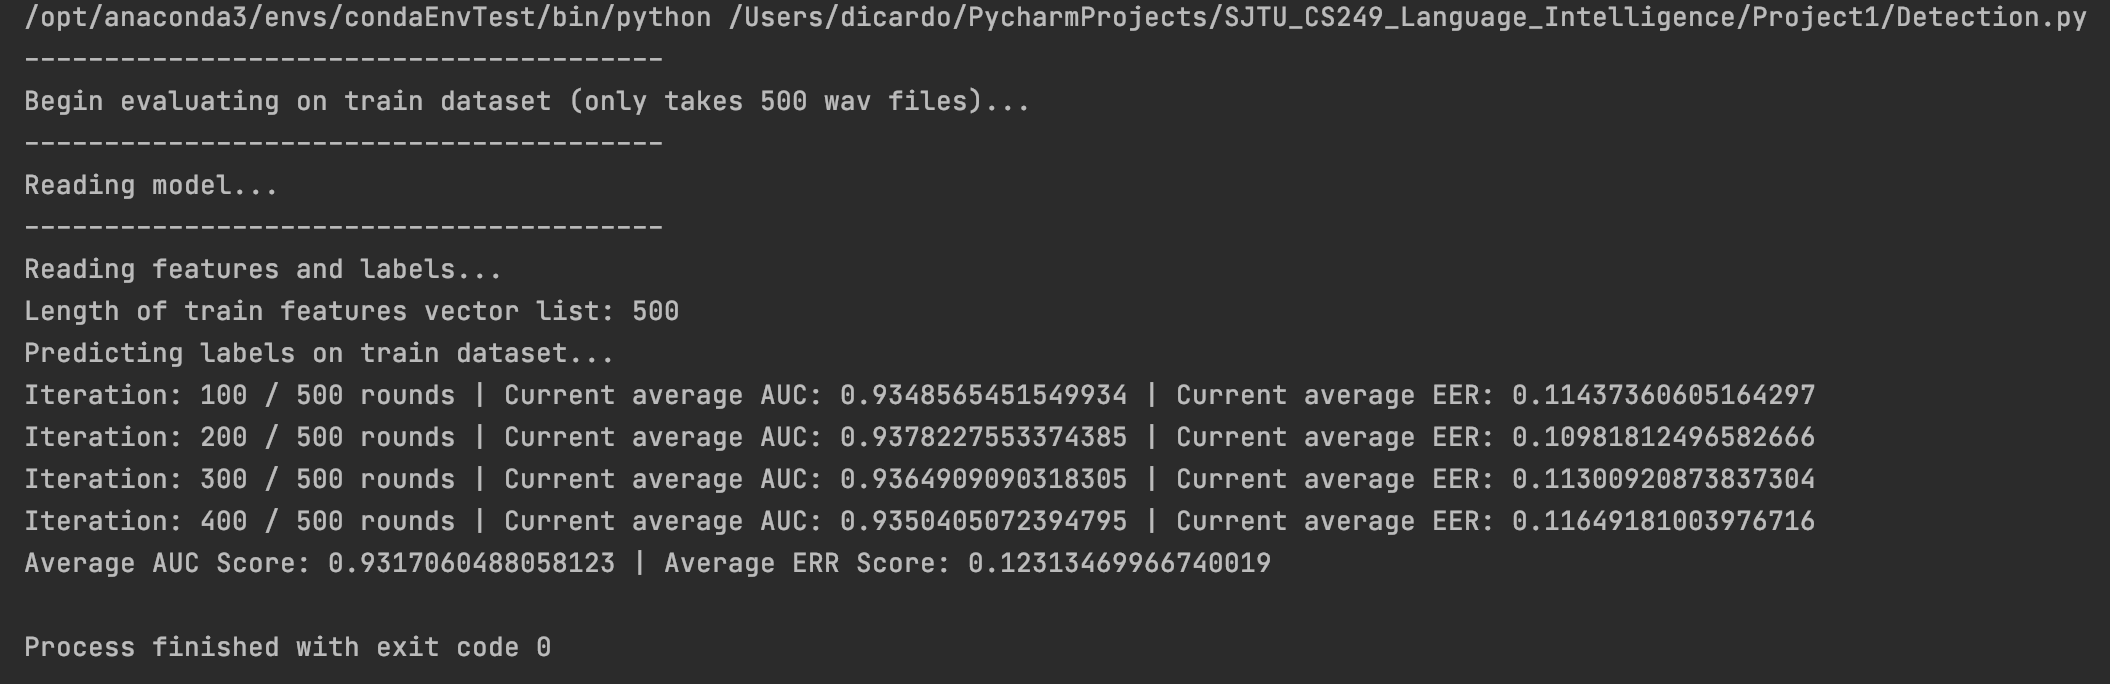
\includegraphics[scale=0.21]{figs/test on train dataset.png}
  \caption{train训练集指标评估结果}
  \label{fig:5}
\end{figure} 

注意到,该结果与直接在dev开发集上评估(AUC 0.9407,EER 0.1044)稍有降低,但在可接受范围内,仍具有很好的模型正确性。

\subsection{基于test测试集的语音端点预测}

本模块对共包含1000个wav样本的test测试集分别进行预处理、特征提取和结果预测,并将预测的结果从以帧为单位转化到以秒为单位,再依据数据集label文件的格式写入到“./output/test\_prediction.txt”目录下,以便后续的测试和评估。通过随机选择一个wav文件,绘制相应的预测结果(如图\ref{fig:6}和\ref{fig:7}),并与对应的wav文件进行人工比较可以大致验证本模型预测的正确性。

\begin{figure}[htb]
  \centering
  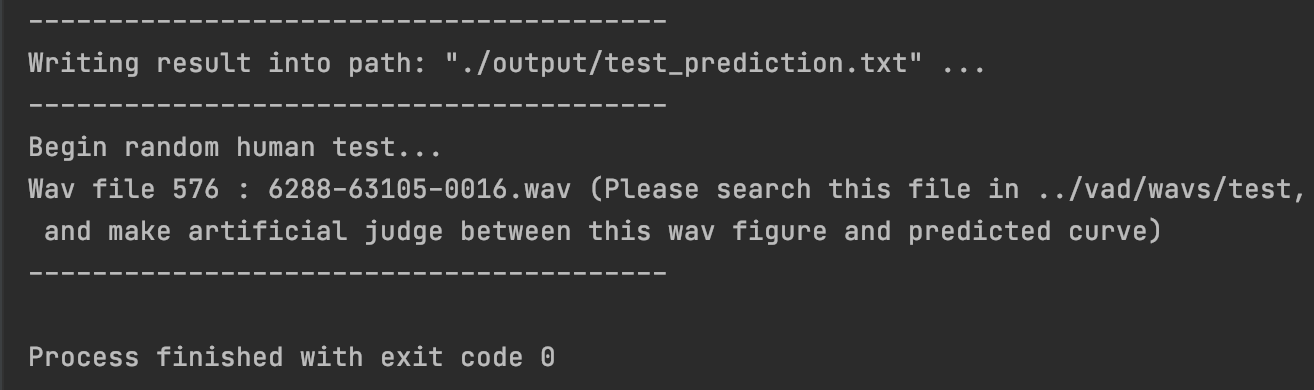
\includegraphics[scale=0.35]{figs/human_test.png}
  \caption{人工检测测试集预测的准确性(1)}
  \label{fig:6}
\end{figure} 

\begin{figure}[htb]
  \centering
  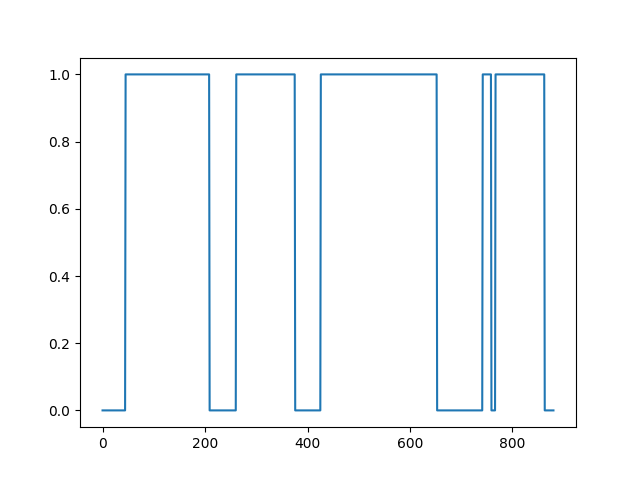
\includegraphics[scale=0.5]{figs/predict.png}
  \caption{人工检测测试集预测的准确性(2)}
  \label{fig:7}
\end{figure} 

\section{总结}

本文提出了一种简单语音端点检测的可行性方案,通过基于语音时域和频域的短时特征构造特征向量,使用Logistic Regression模型构建线性分类器,并利用有限状态机FSM实现语音信号的端点检测。实验结果表明,该模型在少量训练的条件下能够达到很高的预测准确度。

\section{参考文献}

\begin{enumerate}
    \item \label{ref1} J. Ling, S. Sun, J. Zhu and X. Liu, "Speaker Recognition with VAD," 2009 Second Pacific-Asia Conference on Web Mining and Web-based Application, 2009, pp. 313-315, doi: 10.1109/WMWA.2009.59.
\end{enumerate}



\end{document}